\section{Background}\label{sec:ccg}
Language comprehension could be briefly stated as the process of transforming words into meaning. Language production is the opposite process. Language production thus consists of several tasks: idea formation, lexical selection, and grammatical encoding. As it stands, the presented model focuses solely on grammatical encoding, which can also be referred to as constituent assembly. 

\subsection{Linguistic Theory}
\textit{Combinatory Categorial Grammar} (CCG) is a grammatical formalism that makes several psycholinguistic predictions \citep{ccg}. Unlike many grammars, it holds that there are a very few number of actual syntactic rules, but a very large number of syntactic types. Moreover, after a rule is applied, the two syntactic types are combined into a single type. This naturally has fairly direct implications for memory usage in language production: combining things reduces the memory needed to store them. See Figure~\ref{eqn:ccg} for a demonstration of the rules. See Figure~\ref{fig:ccg} for an example of a derivation.

CCG is a grammar in the family of mildly-context sensitive grammars, along with Tree-Adjoining Grammar \citep{tag}. Mildly-context sensitive grammars have been shown to be capable of representing human speech, and computationally plausible in real-time \citep{convergence}. The main difference is that TAG requires the storage of the entire syntactic tree, which has markedly different predictions for memory use during language.

\begin{figure}
\[X/Y > Y = X\]
\[Y < X\setminus Y = X\]
\[X/Y >> Y/Z = X/Z\]
\[Y\setminus Z << X\setminus Y = X\setminus Z\]
\caption{Forward Application, Backward Application, Forward Composition, and Backward Composition respectively. Note that types $A,B$ could be any of combinatorially derived types of CCG}
\label{eqn:ccg}
\end{figure}

\begin{figure}[ht]
\begin{center}
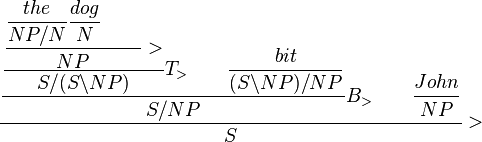
\includegraphics[width=0.95\columnwidth]{figures/ccg}
\end{center}
\caption{An example of a derivation of CCG. Note that the $T>$ is for type-raising, which is handled my declarative memory rather than production rules in my model. \textbf{Redo with my own application combinators}}  
\label{fig:ccg}
\end{figure}

\section{ACT-R}
ACT-R is a general purpose theory of cognition \citep{actr}. From the perspective of a cognitive scientist, ACT-R can be thought of as a theory of memory and learning. From the perspective of the computational modeler, it can be thought of as a set of constraints that one must follow in order to claim cognitive plausibility. Thus, ACT-R, combined with a linguistic theory like CCG, gives us the unification between computational modeling, cognitive science, and linguistics.

ACT-R's basic system for writing models involves chunks and production rules. Chunks make up declarative memory: what you know. Production rules, on the other hand, are simple cognitive operations: they can be thought of as your knowledge of how to do things. Lastly, there are buffers. The two most important buffers are the \textit{retrieval} buffer, which is the interface for accessing declarative memory from the production rules, and the \textit{goal} buffer, which could be thought of as working memory. ACT-R has several mechanisms for learning and decision-making: the most important to this work is \textit{activation}. In short, activation refers to a declarative memory mechanism that keeps track of how recently structures were used and how frequently structures are used in general. Lastly, activation can refer to \textit{spreading activation}, which is the process by which items gain activation in the short term while people are thinking of related items. For instance, after thinking of \textit{spy}, the word \textit{bug} could become more active.

However, most ACT-R models, unlike most computational models, are designed to explain a fairly limited set of data. The models themselves are often hand-coded. This makes empirical evaluation difficult: two separate models are often not comparable. While models often seek to validate themselves with a comparison to experimental data, two separate models might have two separate experiments that they seek to explain. To move beyond this, we suggest the paradigm that, when possible, models be evaluated on large datasets. For the tasks involved in language production, a corpus-based evaluation can help differentiate which models are more accurately performing the task, given cognitive constraints.


\section{Model}
Our model can be thought of in two ways. The first, we see as a novel methodology for implementing and evaluating cognitive models, with a focus on linguistics and language production. From this perspective, the methodology makes only very modest assumptions about how language production works in the mind, leaving the answers to empirical validation. However, due to necessity, we make several assumptions in order to create a model that can answer one question, which provides credibility for the methodology in general.

The presented model is implemented in jACT-R \citep{jactr}, a full Java implementation of the ACT-R theory \citep{actr}. This was primarily due to convenience, portability, and scalability, rather than any difference in theoretical predictions between jACT-R and the core lisp ACT-R. 

The presented model uses CCG, due to its relatively natural mapping to chunks and production rules. The exact mapping will be explained in Sections~\ref{sec:dm} and \ref{sec:rules}.

The model is generated from a corpus. The model's goal is to encode all of the sentences found in the corpus into declarative memory and production rules. In this way, our model could be thought of as a broad range of ACT-R models that can produce a range of sentences; however, from now on, we will refer to the model as a specific model that was experimentally tested. This model learned from a subset of the Switchboard corpus, which is part of the Penn Treebank \cite{treebank}. In order to limit the growth of the model, filters were applied on Switchboard to choose sentences that were shorter and used more common syntactic types. Then, the model learned the words and potential syntactic types from the raw text and CCG annotations. Importantly, nothing besides the CCG types of words was learned from the derivations.

In short, the current model greedily combines lexical-syntactic chunks together to form a sentence. Importantly, it treats no words, types, or rules as special, and it has no knowledge of what words or types should go together beyond the constraints of CCG. 

As many have pointed out (e.g. White), just following these constraints can lead to unidiomatic sentences, and potentially even ungrammatical sentences by violating certain constraints. This is true of the presented model. However, we argue that on the full range of syntactic and lexical constructions found in a corpora, producing idiomatic sentences requires learning, which is out of scope for the present paper. 

\subsection{Declarative Memory}\label{sec:dm}
Declarative Memory is composed of a few simple chunk types, described below. The organizational scheme of the chunks can be found in Figure~\ref{fig:dm}.
\begin{itemize}
\item Word : A word simply has a name, which corresponds to its lexical information (e.g. family).
\item Type : A type is an arbitrarily complicated CCG type. The types that exist in DM are the types that are used in the Switchboard CCG derivations.
\item Lexsyn : A Lexsyn associates a Word with some number of Types. The chosen types are the types that the word has in the Switchboard corpus, including from type-raising. The types are ordered from most common to least common, which would mean more common types would be selected if all else is equal\footnote{Type-raising is a CCG operation where a type changes to a symbolically different but effectively equivalent type. This allows derivations in different orders.}
\item Sentence : As creating a sentence is the goal, sentences are normally in the goal buffer. As described earlier, this could be thought of as working memory. Thus, the sentence contains the current state of grammatical encoding. This workspace can vary in the amount of chunks allowed, which would correspond to different predictions about working memory availability in grammatical encoding. As discussed later, this variation can make a difference in performance. The sentence chunk also contains the input for the task. This is more of a limitation than a theoretical commitment: due to our focus on grammatical encoding, we had to assume the previous tasks of idea generation and lexical selection were complete. In reality, it is likely that all three tasks happen concurrently to some extent.
\end{itemize}

\subsection{Production Rules}\label{sec:rules}
The model's production rules fall into three basic categories: (1) CCG syntax rules, (2) Add/Remove something from Working Memory (the goal buffer), or (3) retrieve something from declarative memory to complete (1) or 92). A general layout of the production rules can be found in Figure~\ref{fig:prod}. The rules are described in more detail as follows.
\begin{itemize}
\item Add a word from the Input to Working Memory: This production rule can only fire if there is space in the goal buffer for it to be added. If so, it initializes a different rule that retrieves the syntactic information about that word, which then adds that to working memory as well.
\item Apply Syntactic Rule between two Lexsyns in Working Memory: This production rule can only fire if Working Memory contains at least two Lexsyns whose types would follow the constraints of at least one CCG rule. This first commits the Lexsyns to a single type, if they were not already committed. Then, it combines these two types into a single type, by initiating a retrieval from declarative memory for that type. Lastly, it clears the now unused slot in Working Memory.
\item Flush: If no other rules apply, the model will flush, clearing its retrieval buffer or working memory to try again. Alternatively, the model could move on to trying to realize a different sentence, if a different sentence is more activated. 
\end{itemize}

\begin{figure}[ht]
\begin{center}
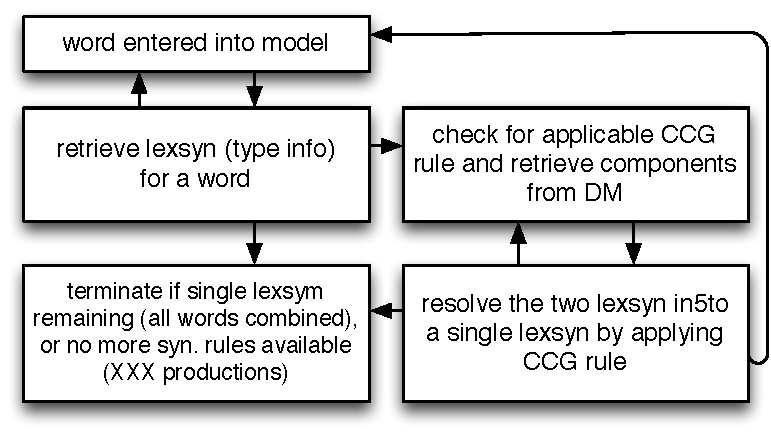
\includegraphics[width=0.95\columnwidth]{figures/model-FSA}
\end{center}
\caption{General process flow of the production rules of the model. See Section~\ref{sec:rules} for a more detailed description.}  
\label{fig:prod}
\end{figure}

\begin{figure}[ht]
\begin{center}
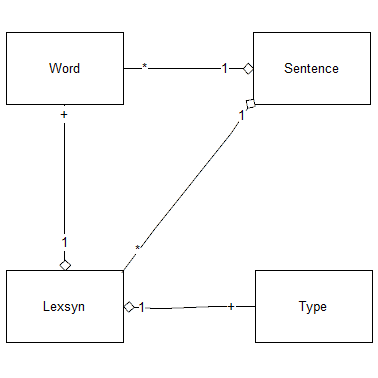
\includegraphics[width=0.95\columnwidth]{figures/prodtypes}
\end{center}
\caption{General data model of the declarative memory. See Section~\ref{sec:dm} for a more detailed description.}  
\label{fig:dm}
\end{figure}

\subsection{Input}
Due to our focus on grammatical encoding, the input to the model was a bag of words generated from a sentence in the Switchboard corpus. 

\subsection{Output}
The model attempts to produce a sentence. However, it does not always successfully finish a sentence, sometimes producing a fragment or several disconnected fragments. In the ideal case, the model would successfully produce the same sentence from which its input was generated, thus emulating (and perhaps simulating) the process of grammatical encoding.



